\documentclass[UTF8,zihao=-4]{ctexart}
\usepackage[teacher]{../../../common/ipara}
\usepackage{mathtools}
\usepackage{pgfplots}
\pgfplotsset{compat=1.18}
\usetikzlibrary{arrows.meta,angles,quotes,positioning,patterns}

\pagestyle{fancy}
\fancyhf{}
\fancyhead[L]{高中数学试卷讲评教师版}
\fancyhead[R]{第 \thepage 页 / 共 \pageref{LastPage} 页}
\renewcommand{\headrulewidth}{0.4pt}

\newcommand{\R}{\mathbb{R}}
\newcommand{\Z}{\mathbb{Z}}
\newcommand{\ans}[1]{\(\boxed{#1}\)}
\newcommand{\qtitle}[2]{%
  \subsection*{第 #1 题\quad #2}
  \addcontentsline{toc}{subsection}{第 #1 题\quad #2}
}
\newcommand{\tightlist}{\setlength{\itemsep}{0.2em}\setlength{\topsep}{0.2em}}

\title{\bfseries 高中数学试卷讲评完整稿\\
\large 选择、填空、解答题系统梳理与方法模型拓展}
\author{教师讲评版}
\date{}

\begin{document}
\maketitle

\begin{teachbox}{讲评定位}
本稿按专题复习课与试卷讲评课合用来编排。处理顺序为：先稳定答案与逻辑，再提炼读题入口，最后补足图像和空间结构。课堂讲评时不建议逐字照读，而应抓住每题的触发条件：看到什么信息，启动什么模型，怎样避免典型失误。
\end{teachbox}

\tableofcontents
\newpage

\section{全卷答案速览与讲评主线}

\begin{center}
\begin{tabularx}{0.95\linewidth}{c|*{8}{>{\centering\arraybackslash}X}}
\toprule
题号 & 1 & 2 & 3 & 4 & 5 & 6 & 7 & 8\\
\midrule
答案 & A & C & B & C & D & B & B & A\\
\bottomrule
\end{tabularx}
\end{center}

\begin{center}
\begin{tabularx}{0.65\linewidth}{c|*{3}{>{\centering\arraybackslash}X}}
\toprule
题号 & 9 & 10 & 11\\
\midrule
答案 & ABD & BC & ACD\\
\bottomrule
\end{tabularx}
\end{center}

\begin{center}
\begin{tabularx}{0.75\linewidth}{c|>{\centering\arraybackslash}X}
\toprule
题号 & 结果\\
\midrule
12 & \(A(2,-6)\)\\
13 & \(\sqrt6\text{ km}\)\\
14 & \(5\sqrt3\pi\)\\
\bottomrule
\end{tabularx}
\end{center}

\begin{center}
\begin{tabularx}{0.95\linewidth}{c|X}
\toprule
题号 & 核心结果\\
\midrule
15 & \(m=2\)，且第（3）问 \(|c|=\sqrt{10}\)\\
16 & \(f(x)=2\sin(2x-\frac{\pi}{3})\)，增区间 \([-\frac{\pi}{12}+k\pi,\frac{5\pi}{12}+k\pi]\)，最大值 \(2\)，最小值 \(-\sqrt3\)\\
17 & \(AC_1\perp CB_1\)，所成角为 \(\frac{\pi}{2}\)\\
18 & \(A=\frac{2\pi}{3}\)，\(AC=\frac{8\sqrt3+4}{11}\)，\(BC\in(2,2\sqrt3]\)\\
19 & \(\cos\angle(C-PB-D)=-\frac1{25}\)，\(|PQ|_{\min}=\frac{6\sqrt{21}}7\)\\
\bottomrule
\end{tabularx}
\end{center}

\begin{teachbox}{本卷讲评主线}
\begin{enumerate}[leftmargin=2em]
  \tightlist
  \item 基础题讲“触发条件”：定义域排除点、外接球找体对角线、向量模平方公式、圆台轴截面。
  \item 图像题讲“从图读参”：先读振幅、周期、零点方向，再写解析式，最后用整体角处理单调与最值。
  \item 空间题讲“降维与基底”：能用平面截面先降维，遇到异面角和线面关系再用平移或空间向量兜底。
  \item 压轴题讲“转化链”：圆周角与线面垂直、二面角平面角、体积比转距离比、空间最值转平面线段最值。
\end{enumerate}
\end{teachbox}

\section{选择题与多选题讲评}

\qtitle{1}{三角函数定义域}

{\small 函数 $f(x)=\tan x$ 的定义域为
\mcoptions[1]{${x\mid x\ne \frac{\pi}{2}+k\pi,\ k\in\mathbb Z}$}{${x\mid x\ne \frac{\pi}{2}+2k\pi,\ k\in\mathbb Z}$}{${x\mid x\ne \pi+k\pi,\ k\in\mathbb Z}$}{${x\mid x\ne \pi+2k\pi,\ k\in\mathbb Z}$}}

\textbf{【解答】}
函数 \(f(x)=\tan x\) 的定义域为
\[
\{x\mid x\ne \frac{\pi}{2}+k\pi,\ k\in\Z\}.
\]
因为 \(\tan x=\frac{\sin x}{\cos x}\)，函数有意义要求 \(\cos x\ne0\)，故必须排除
\[
x=\frac{\pi}{2}+k\pi,\quad k\in\Z.
\]
答案为 \ans{A}。

\begin{teachbox}{易错诊断}
B 项只排除了 \(\frac{\pi}{2}+2k\pi\)，漏掉了 \(\frac{3\pi}{2}+2k\pi\)。讲评时要让学生明确：三角函数定义域不是背选项，而是先找“分母为零”的无意义点。
\end{teachbox}

\qtitle{2}{正方体外接球}

{\small 棱长为 $2$ 的正方体的 $8$ 个顶点都在球 $O$ 的表面上，则球 $O$ 的半径为
\mcoptions[1]{$1$}{$\sqrt2$}{$\sqrt3$}{$2$}}

\textbf{【解答】}
棱长为 \(2\) 的正方体的外接球半径等于体对角线的一半：
\[
d=\sqrt{2^2+2^2+2^2}=2\sqrt3,\qquad R=\frac d2=\sqrt3.
\]
答案为 \ans{C}。

\begin{center}
\begin{tikzpicture}[scale=0.85,line cap=round,line join=round]
  \coordinate (A) at (0,0);
  \coordinate (B) at (2.2,0);
  \coordinate (D) at (-0.75,0.75);
  \coordinate (C) at (1.45,0.75);
  \coordinate (A1) at (0,2.2);
  \coordinate (B1) at (2.2,2.2);
  \coordinate (D1) at (-0.75,2.95);
  \coordinate (C1) at (1.45,2.95);
  \draw (A)--(B)--(C);
  \draw[dashed] (C)--(D)--(A);
  \draw (A1)--(B1)--(C1)--(D1)--cycle;
  \draw (A)--(A1) (B)--(B1) (C)--(C1);
  \draw[dashed] (D)--(D1);
  \draw[thick] (A)--(C1);
  \fill (0.725,1.475) circle (1.5pt) node[right] {\small 球心};
  \node[below left] at (A) {\small \(A\)};
  \node[above right] at (C1) {\small \(C_1\)};
  \node at (1.2,1.3) {\small \(R=\frac12 AC_1\)};
\end{tikzpicture}

{\small 图 1：正方体外接球半径即体对角线的一半。}
\end{center}

\qtitle{3}{两边夹角求面积}

{\small 在 $\triangle ABC$ 中，$AB=4$，$AC=3$，$\angle BAC=\frac{\pi}{6}$，则 $\triangle ABC$ 的面积为
\mcoptions[1]{$2$}{$3$}{$4$}{$6$}}

\textbf{【解答】}
已知 \(AB=4\)，\(AC=3\)，\(\angle BAC=\frac{\pi}{6}\)，直接用夹角面积公式：
\[
S_{\triangle ABC}=\frac12\cdot AB\cdot AC\cdot \sin\angle BAC
=\frac12\cdot4\cdot3\cdot\frac12=3.
\]
答案为 \ans{B}。

\qtitle{4}{圆锥与球的表面积比}

{\small 若圆锥的底面直径和母线都等于球的直径，则圆锥与球的表面积之比为
\mcoptions[1]{$\frac23$}{$\frac2\pi$}{$\frac34$}{$\frac4\pi$}}

\textbf{【解答】}
设球半径为 \(R\)，则球直径为 \(2R\)。题意给出圆锥底面直径和母线都等于球直径，故圆锥底面半径 \(r=R\)，母线 \(l=2R\)。圆锥表面积为
\[
S_{\text{锥}}=\pi r^2+\pi rl=\pi R^2+2\pi R^2=3\pi R^2,
\]
球表面积为 \(S_{\text{球}}=4\pi R^2\)，故
\[
\frac{S_{\text{锥}}}{S_{\text{球}}}=\frac34.
\]
答案为 \ans{C}。

\begin{teachbox}{讲评提醒}
题目问“圆锥表面积”，默认包含底面积与侧面积。若只算侧面积，会把 \(\pi rl\) 当成全部，得到错误比例。
\end{teachbox}

\qtitle{5}{单位向量夹角}

{\small 若单位向量 $e_1,e_2$ 满足 $|e_1+e_2|=1$，则 $e_1,e_2$ 的夹角为
\mcoptions[1]{$\frac{\pi}{6}$}{$\frac{\pi}{3}$}{$\frac{\pi}{2}$}{$\frac{2\pi}{3}$}}

\textbf{【解答】}
设两个单位向量 \(e_1,e_2\) 的夹角为 \(\theta\)。由
\[
|e_1+e_2|^2=|e_1|^2+|e_2|^2+2e_1\cdot e_2
\]
得
\[
1=1+1+2\cos\theta,\qquad \cos\theta=-\frac12.
\]
向量夹角满足 \(0\le \theta\le\pi\)，所以 \(\theta=\frac{2\pi}{3}\)。答案为 \ans{D}。

\begin{teachbox}{追问}
若学生选 \(\frac{\pi}{3}\)，追问：“等边三角形的内角”和“两个向量从同一起点出发的夹角”是不是同一个角？这一步能纠正大量凭图直觉误判。
\end{teachbox}

\qtitle{6}{圆台体积}

{\small 已知圆台的上、下底面半径分别为 $1$ 和 $2$，且圆台的母线与一底面所成的角为 $\frac{\pi}{4}$，则圆台的体积为
\mcoptions[1]{$\frac{4\pi}{3}$}{$\frac{7\pi}{3}$}{$\frac{5\pi}{2}$}{$3\pi$}}

\textbf{【解答】}
圆台上、下底面半径分别为 \(1,2\)，母线与底面成 \(\frac{\pi}{4}\)。在轴截面中，高 \(h\) 与半径差 \(R-r=1\) 构成直角三角形：
\[
\tan\frac{\pi}{4}=\frac{h}{R-r}=h,\qquad h=1.
\]
故
\[
V=\frac13\pi h(R^2+Rr+r^2)
=\frac13\pi(2^2+2\cdot1+1^2)=\frac{7\pi}{3}.
\]
答案为 \ans{B}。

\begin{center}
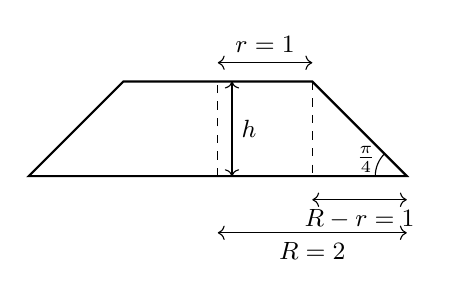
\begin{tikzpicture}[scale=1.2]
  \coordinate (A) at (-2,0);
  \coordinate (B) at (2,0);
  \coordinate (C) at (1,1);
  \coordinate (D) at (-1,1);
  \coordinate (O) at (0,0);
  \coordinate (O1) at (0,1);
  \coordinate (H) at (1,0);
  
  \draw[thick] (A)--(B)--(C)--(D)--cycle;
  \draw[dashed] (O)--(O1);
  \draw[dashed] (C)--(H);
  
  \draw[<->] (0,-0.6)--(2,-0.6) node[midway,below] {\small \(R=2\)};
  \draw[<->] (0,1.2)--(1,1.2) node[midway,above] {\small \(r=1\)};
  \draw[<->] (1,-0.25)--(2,-0.25) node[midway,below] {\small \(R-r=1\)};
  \draw[<->] (0.15,0)--(0.15,1) node[midway,right] {\small \(h\)};
  
  \draw pic["\small \(\frac{\pi}{4}\)",draw,angle radius=0.4cm,angle eccentricity=1.4] {angle=C--B--A};
\end{tikzpicture}

{\small 图 2：圆台轴截面把立体体积题降为直角三角形。}
\end{center}

\qtitle{7}{正方体中的平面交线与线线角}

{\small 在正方体 $ABCD-A_1B_1C_1D_1$ 中，过直线 $AA_1$ 且平行于平面 $BDD_1B_1$ 的平面 $\alpha$ 交平面 $ACD_1$ 于直线 $l$，则直线 $AA_1$ 与 $l$ 所成角的正切值为
\mcoptions[1]{$\frac12$}{$\frac{\sqrt2}{2}$}{$\sqrt2$}{$2$}}

\textbf{【解答】}
设正方体棱长为 \(1\)，取
\[
\overrightarrow{AB}=\mathbf i,\quad \overrightarrow{AD}=\mathbf j,\quad \overrightarrow{AA_1}=\mathbf k.
\]
平面 \(BDD_1B_1\) 由方向 \(\mathbf j-\mathbf i\) 与 \(\mathbf k\) 张成。因此过 \(AA_1\) 且平行于该平面的平面 \(\alpha\) 内任意交线方向可写成
\[
\mathbf v=s(\mathbf j-\mathbf i)+t\mathbf k=-s\mathbf i+s\mathbf j+t\mathbf k.
\]
又平面 \(ACD_1\) 由 \(\mathbf i+\mathbf j\) 与 \(\mathbf j+\mathbf k\) 张成，故同一方向也可写成
\[
\mathbf v=m(\mathbf i+\mathbf j)+n(\mathbf j+\mathbf k)
=m\mathbf i+(m+n)\mathbf j+n\mathbf k.
\]
比较系数：
\[
m=-s,\quad m+n=s,\quad n=t,
\]
得 \(n=2s,t=2s\)，故可取
\[
\mathbf v=-\mathbf i+\mathbf j+2\mathbf k.
\]
直线 \(AA_1\) 的方向为 \(\mathbf k\)。\(\mathbf v\) 的水平分量长为 \(\sqrt2\)，竖直分量长为 \(2\)，所以
\[
\tan\theta=\frac{\sqrt2}{2}.
\]
答案为 \ans{B}。

\begin{center}
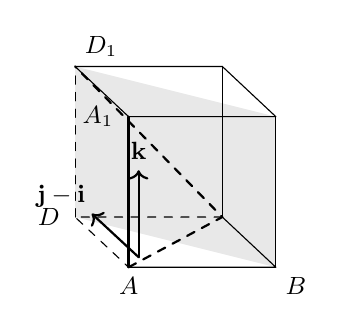
\begin{tikzpicture}[scale=0.85,line cap=round,line join=round]
  \coordinate (A) at (0,0);
  \coordinate (B) at (2.2,0);
  \coordinate (D) at (-0.8,0.75);
  \coordinate (C) at (1.4,0.75);
  \coordinate (A1) at (0,2.25);
  \coordinate (B1) at (2.2,2.25);
  \coordinate (D1) at (-0.8,3.0);
  \coordinate (C1) at (1.4,3.0);
  \fill[gray!18] (B)--(D)--(D1)--(B1)--cycle;
  \draw (A)--(B)--(C);
  \draw[dashed] (C)--(D)--(A);
  \draw (A1)--(B1)--(C1)--(D1)--cycle;
  \draw (A)--(A1) (B)--(B1) (C)--(C1);
  \draw[dashed] (D)--(D1);
  \draw[thick] (A)--(A1);
  \draw[thick,dashed] (A)--(C)--(D1);
  \draw[thick,->] (0.15,0.15)--(-0.55,0.8) node[above left=-2pt] {\small \(\mathbf j-\mathbf i\)};
  \draw[thick,->] (0.15,0.15)--(0.15,1.45) node[above] {\small \(\mathbf k\)};
  \node[below] at (A) {\small \(A\)};
  \node[below right] at (B) {\small \(B\)};
  \node[left=2pt] at (D) {\small \(D\)};
  \node[left=2pt] at (A1) {\small \(A_1\)};
  \node[above right] at (D1) {\small \(D_1\)};
\end{tikzpicture}

{\small 图 3：把平面平行与交线方向转成三个棱方向的线性组合。}
\end{center}

\begin{teachbox}{讲评重点}
本题不是“画出交线”最难，而是把“交线在两个平面内”翻译成“同一个向量有两种表示”。讲评时可先问：平面 \(ACD_1\) 中能选哪两个不共线方向？平面 \(\alpha\) 又继承了哪两个方向？
\end{teachbox}

\qtitle{8}{和差化积与三角形内角和}

{\small 在 $\triangle ABC$ 中，若

$$  
A-B=\frac{\pi}{3},  
$$

且

$$  
\sin A+\sin B=1,  
$$

则 $\cos C=$
\mcoptions[1]{$-\frac13$}{$\frac13$}{$-\frac79$}{$\frac79$}}

\textbf{【解答】}
由和差化积：
\[
\sin A+\sin B=2\sin\frac{A+B}{2}\cos\frac{A-B}{2}.
\]
已知 \(A-B=\frac{\pi}{3}\)，故
\[
1=\sin A+\sin B=\sqrt3\sin\frac{A+B}{2},
\]
即 \(\sin\frac{A+B}{2}=\frac1{\sqrt3}\)。设 \(S=A+B\)，则
\[
\cos S=1-2\sin^2\frac S2=1-\frac23=\frac13.
\]
又 \(C=\pi-S\)，故
\[
\cos C=\cos(\pi-S)=-\cos S=-\frac13.
\]
答案为 \ans{A}。

\qtitle{9}{三角函数图象性质}

{\small 已知函数

$$  
f(x)=\cos\left(2x+\frac{\pi}{4}\right)+1,  
$$

则
\mcoptions[1]{$f(x)$ 的最小正周期为 $\pi$}{$f(x)$ 的对称中心为 $\left(\frac{\pi}{8}+\frac{k\pi}{2},1\right),\ k\in\mathbb Z$}{$f(x)$ 的对称轴为 $x=\frac{5\pi}{8}+\frac{k\pi}{2},\ k\in\mathbb Z$}{方程 $f(x)=1$ 在区间 $[0,\pi]$ 上恰有两根}}

\textbf{【解答】}
已知
\[
f(x)=\cos\left(2x+\frac{\pi}{4}\right)+1.
\]
周期 \(T=\frac{2\pi}{2}=\pi\)，A 正确。对称中心满足
\[
2x+\frac{\pi}{4}=\frac{\pi}{2}+k\pi,
\]
故
\[
\left(\frac{\pi}{8}+\frac{k\pi}{2},1\right)
\]
是对称中心，B 正确。对称轴满足
\[
2x+\frac{\pi}{4}=k\pi,\qquad x=-\frac{\pi}{8}+\frac{k\pi}{2},
\]
与选项 C 不同，C 错误。方程 \(f(x)=1\) 得
\[
x=\frac{\pi}{8}+\frac{k\pi}{2}.
\]
在 \([0,\pi]\) 上取 \(k=0,1\)，恰有两根，D 正确。答案为 \ans{ABD}。

\begin{center}
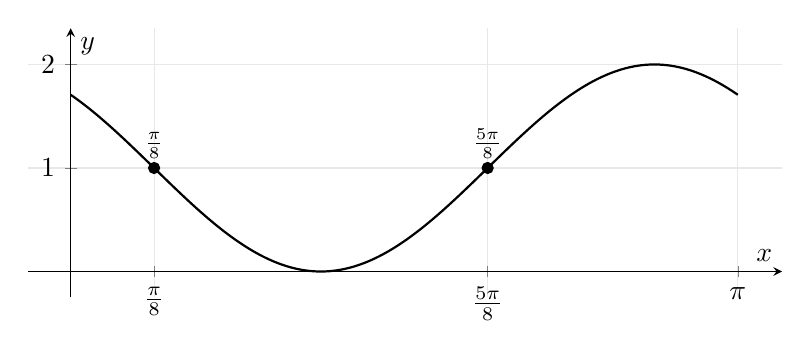
\begin{tikzpicture}
\begin{axis}[
  width=0.92\linewidth,height=5.0cm,
  axis lines=middle,
  xmin=-0.2,xmax=3.35,ymin=-0.25,ymax=2.35,
  xtick={0,0.3927,1.9635,3.1416},
  xticklabels={$0$,$\frac{\pi}{8}$,$\frac{5\pi}{8}$,$\pi$},
  ytick={0,1,2},
  grid=both,
  grid style={gray!18},
  domain=0:3.1416,
  samples=220,
  xlabel={$x$},ylabel={$y$}
]
\addplot[black,thick] {cos(deg(2*x+pi/4))+1};
\addplot[only marks,mark=*] coordinates {(0.3927,1) (1.9635,1)};
\node[above] at (axis cs:0.3927,1) {\small \(\frac{\pi}{8}\)};
\node[above] at (axis cs:1.9635,1) {\small \(\frac{5\pi}{8}\)};
\end{axis}
\end{tikzpicture}

{\small 图 4：对称中心落在中线 \(y=1\) 上，方程 \(f(x)=1\) 即求中线交点。}
\end{center}

\qtitle{10}{空间线面位置关系}

{\small 已知 $\alpha,\beta$ 是两个不同的平面，$a,b$ 是两条不同的直线，下列命题正确的是
\mcoptions[1]{若 $a\parallel b,\ b\subset\beta,\ \alpha\parallel\beta$，则 $a\parallel\alpha$}{若 $a\parallel\alpha,\ a\subset\beta,\ \alpha\cap\beta=b$，则 $a\parallel b$}{若 $a\perp\alpha,\ b\perp\beta,\ a\perp b$，则 $\alpha\perp\beta$}{若 $\alpha\perp\beta,\ a\subset\alpha,\ b\subset\beta$，则 $a\perp b$}}

\textbf{【解答】}
\begin{enumerate}[leftmargin=2em]
  \tightlist
  \item A 错。若 \(a\subset\alpha\) 且 \(a\parallel b\)，虽然满足前提，但不能称 \(a\parallel\alpha\)。
  \item B 对。\(a,b\) 同在 \(\beta\) 内；若 \(a\) 与 \(b\) 相交，则交点在 \(\alpha\) 上，与 \(a\parallel\alpha\) 矛盾，故 \(a\parallel b\)。
  \item C 对。两条直线分别为两平面的法线，法线垂直推出平面垂直。
  \item D 错。两个平面垂直，不代表分别在两平面内的任意两线都垂直。可取 \(a\parallel\alpha\cap\beta\)，\(b=\alpha\cap\beta\)，则 \(a\parallel b\)。
\end{enumerate}
答案为 \ans{BC}。

\qtitle{11}{平面向量综合}

{\small 在 $\triangle ABC$ 中，已知

$$  
\angle BAC=\frac{\pi}{2},\qquad AB=AC.  
$$

$D$ 是 $AC$ 的中点，若 $P$ 是 $BC$ 上一点，且满足

$$  
\overrightarrow{BP}=2\overrightarrow{PC},  
$$

$AP$ 与 $BD$ 交于点 $E$，则
\mcoptions[1]{$\overrightarrow{AP}=\frac13\overrightarrow{AB}+\frac23\overrightarrow{AC}$}{$\overrightarrow{AP}$ 在 $\overrightarrow{AB}$ 上的投影向量为 $\frac23\overrightarrow{AB}$}{$\overrightarrow{AP}\cdot\overrightarrow{BD}=0$}{$\overrightarrow{AE}=\frac35\overrightarrow{AP}$}}

\textbf{【解答】}
设
\[
\overrightarrow{AB}=\mathbf u,\qquad \overrightarrow{AC}=\mathbf v,
\]
则 \(\mathbf u\perp\mathbf v\)，\(|\mathbf u|=|\mathbf v|\)。由 \(\overrightarrow{BP}=2\overrightarrow{PC}\) 得
\[
\overrightarrow{AP}=\mathbf u+\frac23(\mathbf v-\mathbf u)
=\frac13\mathbf u+\frac23\mathbf v,
\]
故 A 正确。

投影向量为
\[
\operatorname{proj}_{\mathbf u}\overrightarrow{AP}
=\frac{\overrightarrow{AP}\cdot\mathbf u}{\mathbf u\cdot\mathbf u}\mathbf u
=\frac13\mathbf u,
\]
不是 \(\frac23\mathbf u\)，B 错误。

又 \(D\) 是 \(AC\) 中点，
\[
\overrightarrow{BD}=\frac12\mathbf v-\mathbf u.
\]
于是
\[
\overrightarrow{AP}\cdot\overrightarrow{BD}
=\left(\frac13\mathbf u+\frac23\mathbf v\right)\cdot\left(\frac12\mathbf v-\mathbf u\right)
=-\frac13|\mathbf u|^2+\frac13|\mathbf v|^2=0,
\]
C 正确。

设 \(\overrightarrow{AE}=\lambda\overrightarrow{AP}\)，又 \(E\in BD\)，则
\[
\lambda\left(\frac13\mathbf u+\frac23\mathbf v\right)
=(1-\mu)\mathbf u+\frac{\mu}{2}\mathbf v.
\]
比较系数：
\[
\frac{\lambda}{3}=1-\mu,\qquad \frac{2\lambda}{3}=\frac{\mu}{2}.
\]
解得 \(\lambda=\frac35\)，D 正确。答案为 \ans{ACD}。

\begin{center}
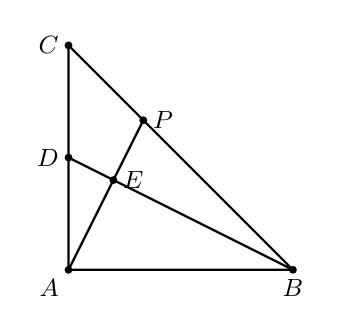
\begin{tikzpicture}[scale=0.95,line cap=round,line join=round]
  \coordinate (A) at (0,0);
  \coordinate (B) at (3,0);
  \coordinate (C) at (0,3);
  \coordinate (D) at (0,1.5);
  \coordinate (P) at (1,2);
  \coordinate (E) at (0.6,1.2);
  \draw[thick] (A)--(B)--(C)--cycle;
  \draw[thick] (B)--(D);
  \draw[thick] (A)--(P);
  \fill (A) circle (1.5pt) node[below left] {\small \(A\)};
  \fill (B) circle (1.5pt) node[below] {\small \(B\)};
  \fill (C) circle (1.5pt) node[left] {\small \(C\)};
  \fill (D) circle (1.5pt) node[left] {\small \(D\)};
  \fill (P) circle (1.5pt) node[right] {\small \(P\)};
  \fill (E) circle (1.5pt) node[right] {\small \(E\)};
  
\end{tikzpicture}

{\small 图 5：选 \(\overrightarrow{AB},\overrightarrow{AC}\) 为基底，分点、投影、垂直、交点统一处理。}
\end{center}

\section{填空题讲评}

\qtitle{12}{向量坐标}

{\small 在平面直角坐标系中，已知点 $B$ 的坐标为 $(4,-3)$，若

$$  
\overrightarrow{AB}=(2,3),  
$$

则点 $A$ 的坐标为\blank{2cm}。}

\textbf{【解答】}
设 \(A(x,y)\)。由
\[
\overrightarrow{AB}=(x_B-x_A,\ y_B-y_A)=(4-x,-3-y)=(2,3)
\]
得 \(x=2,y=-6\)，故 \(A(2,-6)\)。

\qtitle{13}{测距问题}

{\small 在岸边选取相距 $2\text{ km}$ 的 $A,B$ 两点，测得

$$  
\angle DAC=60^\circ,\quad \angle CAB=45^\circ,  
$$

$$  
\angle DBA=30^\circ,\quad \angle DBC=60^\circ.  
$$

求 $CD$。}

\textbf{【解答】}
在 \(\triangle ABC\) 中，\(\angle CAB=45^\circ\)，由题意 \(\angle ABC=30^\circ+60^\circ=90^\circ\)，故 \(\angle ACB=45^\circ\)，且 \(AB=2\)，于是
\[
AC=2\sqrt2.
\]
在 \(\triangle ABD\) 中，
\[
\angle DAB=60^\circ+45^\circ=105^\circ,\qquad \angle DBA=30^\circ,
\]
故 \(\angle ADB=45^\circ\)。由正弦定理
\[
\frac{AD}{\sin30^\circ}=\frac{AB}{\sin45^\circ},
\]
得 \(AD=\sqrt2\)。在 \(\triangle ACD\) 中，\(\angle CAD=60^\circ\)，由余弦定理
\[
CD^2=AC^2+AD^2-2AC\cdot AD\cos60^\circ=8+2-4=6.
\]
因此 \(CD=\sqrt6\text{ km}\)。

\begin{center}
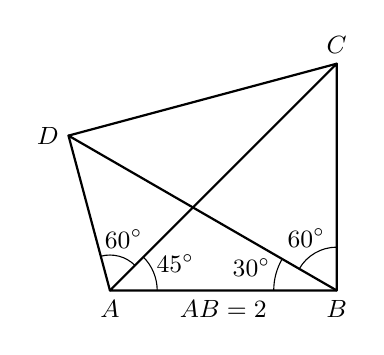
\begin{tikzpicture}[scale=0.9,line cap=round,line join=round]
  \coordinate (A) at (0,0);
  \coordinate (B) at (3.2,0);
  \coordinate (C) at (3.2,3.2);
  \coordinate (D) at (-0.585,2.185);
  \draw[thick] (A)--(B)--(C)--cycle;
  \draw[thick] (A)--(D)--(B);
  \draw[thick] (C)--(D);
  \node[below] at (A) {\small \(A\)};
  \node[below] at (B) {\small \(B\)};
  \node[above] at (C) {\small \(C\)};
  \node[left] at (D) {\small \(D\)};
  \node[below] at (1.6,0) {\small \(AB=2\)};
  \draw pic["\small \(45^\circ\)",draw,angle radius=0.6cm,angle eccentricity=1.5] {angle=B--A--C};
  \draw pic["\small \(60^\circ\)",draw,angle radius=0.45cm,angle eccentricity=1.5] {angle=C--A--D};
  \draw pic["\small \(30^\circ\)",draw,angle radius=0.8cm,angle eccentricity=1.4] {angle=D--B--A};
  \draw pic["\small \(60^\circ\)",draw,angle radius=0.55cm,angle eccentricity=1.4] {angle=C--B--D};
\end{tikzpicture}

{\small 图 6：测距题先把角度合并到两个三角形中。}
\end{center}

\qtitle{14}{球面与正四面体表面的交线}

{\small 以点 $O$ 为球心，半径为 $3\sqrt3$ 的球的表面与以点 $O$ 为顶点、棱长为 $6$ 的正四面体表面的交线为 $P$，则 $P$ 的总长度为\blank{2cm}。}

\textbf{【解答】}
设正四面体为 \(OABC\)，棱长 \(6\)，球心为 \(O\)，球半径 \(R=3\sqrt3\)。

在每个侧面如 \(\triangle OAB\) 中，交线是以 \(O\) 为圆心、半径 \(3\sqrt3\)、圆心角 \(60^\circ=\frac{\pi}{3}\) 的圆弧，一段弧长为
\[
3\sqrt3\cdot\frac{\pi}{3}=\sqrt3\pi.
\]
三个侧面总长为 \(3\sqrt3\pi\)。

正四面体高为
\[
h=6\sqrt{\frac23}=2\sqrt6.
\]
球面与底面 \(ABC\) 所在平面相交的圆半径为
\[
r=\sqrt{(3\sqrt3)^2-(2\sqrt6)^2}=\sqrt3.
\]
边长为 \(6\) 的等边三角形内切圆半径也是 \(\sqrt3\)，故底面交线为内切圆，周长为 \(2\sqrt3\pi\)。总长为
\[
3\sqrt3\pi+2\sqrt3\pi=5\sqrt3\pi.
\]

\begin{center}
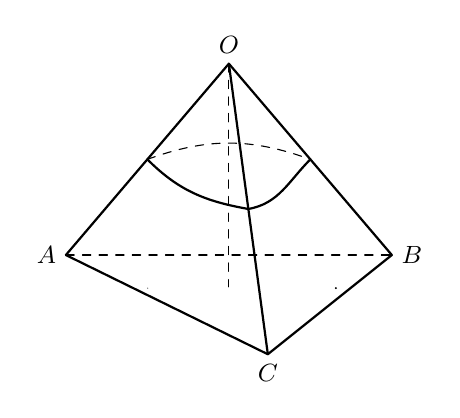
\begin{tikzpicture}[scale=0.9,line cap=round,line join=round]
  \coordinate (O) at (0,2.7);
  \coordinate (A) at (-2.3,0);
  \coordinate (B) at (2.3,0);
  \coordinate (C) at (0.55,-1.4);
  \draw[thick] (A)--(O)--(B);
  \draw[thick] (O)--(C);
  \draw[thick] (A)--(C)--(B);
  \draw[dashed] (A)--(B);
  \draw[dashed] (O)--(0,-0.45);
  \draw[thick] (-1.15, 1.35) to[out=-45, in=170] (0.275, 0.65) to[out=10, in=-135] (1.15, 1.35);
  \draw[dashed] (-1.15, 1.35) to[out=20, in=160] (1.15, 1.35);
  \draw[thick] (0.183,-0.467) ++(1.328,0) arc[start angle=0, end angle=180, x={(1.328cm,0cm)}, y={(0.183cm,-0.467cm)}];
  \draw[dashed] (0.183,-0.467) ++(-1.328,0) arc[start angle=180, end angle=360, x={(1.328cm,0cm)}, y={(0.183cm,-0.467cm)}];
  \node[above] at (O) {\small \(O\)};
  \node[left] at (A) {\small \(A\)};
  \node[right] at (B) {\small \(B\)};
  \node[below] at (C) {\small \(C\)};
\end{tikzpicture}

{\small 图 7：交线由三个侧面圆弧和一个底面整圆组成。}
\end{center}

\section{解答题讲评}

\qtitle{15}{平面向量}

{\small 已知平面向量

$$  
a=(2,1),\qquad b=(m-2,4-2m),\qquad c=a+b.  
$$

（1）若 $a\parallel b$，求实数 $m$ 的值；

（2）证明：对任意 $\lambda\ne0$，都有

$$  
a\perp \lambda(a-c);  
$$

（3）若 $a$ 与 $c$ 的夹角为 $\frac{\pi}{4}$，求 $|c|$。}

\begin{paracol}{2}
\teachblock{标准解答}{
已知
\[
a=(2,1),\qquad b=(m-2,4-2m),\qquad c=a+b.
\]

\textbf{（1）求 \(m\)。} 由 \(a\parallel b\) 得
\[
2(4-2m)-1(m-2)=0,
\]
即 \(10-5m=0\)，故 \(m=2\)。此时 \(b=(0,0)\)，按高中常用约定零向量与任意向量平行。

\textbf{（2）证明垂直。} 因为 \(c=a+b\)，所以
\[
a-c=-b,\qquad \lambda(a-c)=-\lambda b.
\]
只需证 \(a\perp b\)。计算
\[
a\cdot b=2(m-2)+(4-2m)=0.
\]
故 \(a\perp b\)，从而对任意 \(\lambda\ne0\)，有
\[
a\perp \lambda(a-c).
\]

\textbf{（3）求 \(|c|\)。} 由 \(a\perp b\) 且 \(c=a+b\)，得
\[
a\cdot c=a\cdot(a+b)=|a|^2=5.
\]
又 \(|a|=\sqrt5\)，且 \(a\) 与 \(c\) 的夹角为 \(\frac{\pi}{4}\)，所以
\[
5=|a||c|\cos\frac{\pi}{4}
=\sqrt5\,|c|\,\frac{\sqrt2}{2},
\]
故
\[
|c|=\sqrt{10}.
\]
}
\switchcolumn
\teachblock{板书建议}{
第（2）问不要直接写“显然垂直”。先写 \(a-c=-b\)，再算 \(a\cdot b=0\)。这样第（3）问才能自然接上 \(a\cdot c=|a|^2\)。
}
\end{paracol}

\qtitle{16}{三角函数图象}

{\small 已知函数

$$  
f(x)=A\sin(\omega x+\varphi),  
$$

其中

$$  
x\in\mathbb R,\quad A>0,\quad \omega>0,\quad |\varphi|<\frac{\pi}{2}.  
$$

图象如题图。

（1）求 $f(x)$ 的解析式；

（2）求 $f(x)$ 的单调递增区间及 $f(x)$ 在 $[0,\frac{\pi}{2}]$ 上的最大值与最小值。}

\begin{paracol}{2}
\teachblock{标准解答}{
已知
\[
f(x)=A\sin(\omega x+\varphi),\qquad A>0,\quad \omega>0,\quad |\varphi|<\frac{\pi}{2}.
\]
图像给出最大值 \(2\)，并且两个相邻零点为 \(x=\frac{\pi}{6}\)、\(x=\frac{2\pi}{3}\)。

\begin{center}
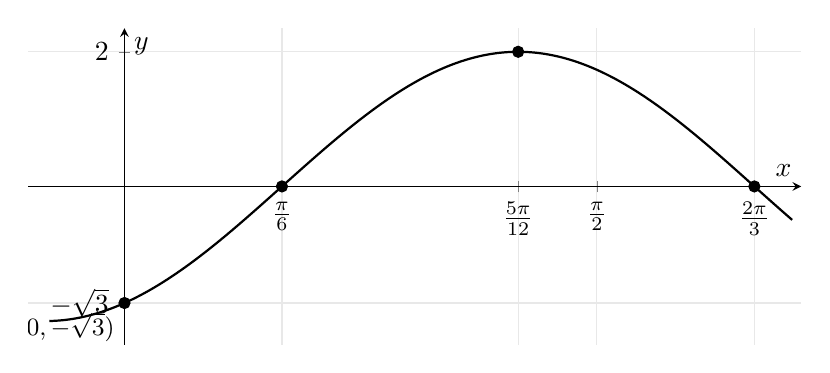
\begin{tikzpicture}
\begin{axis}[
  width=0.94\linewidth,height=5.6cm,
  axis lines=middle,
  xmin=-0.32,xmax=2.25,ymin=-2.35,ymax=2.35,
  xtick={0,0.5236,1.3090,1.5708,2.0944},
  xticklabels={$0$,$\frac{\pi}{6}$,$\frac{5\pi}{12}$,$\frac{\pi}{2}$,$\frac{2\pi}{3}$},
  ytick={-1.732,0,2},
  yticklabels={$-\sqrt3$,$0$,$2$},
  grid=both,
  grid style={gray!18},
  domain=-0.25:2.22,
  samples=260,
  xlabel={$x$},ylabel={$y$}
]
\addplot[black,thick] {2*sin(deg(2*x-pi/3))};
\addplot[only marks,mark=*] coordinates {(0, -1.732) (0.5236,0) (1.3090,2) (2.0944,0)};
\node[below left] at (axis cs:0,-1.732) {\small \((0,-\sqrt3)\)};

\end{axis}
\end{tikzpicture}

{\small 图 8：按原题图信息重构的函数图像。零点方向用于确定相位。}
\end{center}

\textbf{（1）求解析式。} 最大值为 \(2\)，所以 \(A=2\)。相邻零点间距为半个周期：
\[
\frac T2=\frac{2\pi}{3}-\frac{\pi}{6}=\frac{\pi}{2},
\qquad T=\pi.
\]
由 \(T=\frac{2\pi}{\omega}\)，得 \(\omega=2\)。于是
\[
f(x)=2\sin(2x+\varphi).
\]
图像在 \(x=\frac{\pi}{6}\) 处从负到正穿过 \(x\) 轴，对应正弦整体角 \(0\)，故
\[
2\cdot\frac{\pi}{6}+\varphi=0,\qquad \varphi=-\frac{\pi}{3}.
\]
因此
\[
\boxed{f(x)=2\sin\left(2x-\frac{\pi}{3}\right)}.
\]

\textbf{（2）单调区间与最值。} 令 \(t=2x-\frac{\pi}{3}\)。因为 \(\sin t\) 在
\[
\left[-\frac{\pi}{2}+2k\pi,\frac{\pi}{2}+2k\pi\right]
\]
上单调递增，所以
\[
-\frac{\pi}{2}+2k\pi\le 2x-\frac{\pi}{3}\le \frac{\pi}{2}+2k\pi.
\]
解得增区间为
\[
\boxed{\left[-\frac{\pi}{12}+k\pi,\frac{5\pi}{12}+k\pi\right],\quad k\in\Z.}
\]

当 \(x\in[0,\frac{\pi}{2}]\) 时，
\[
t=2x-\frac{\pi}{3}\in\left[-\frac{\pi}{3},\frac{2\pi}{3}\right].
\]
该区间内 \(\sin t\) 最大值为 \(1\)，故 \(f_{\max}=2\)；最小值在左端点 \(t=-\frac{\pi}{3}\) 处取得，故
\[
f(0)=2\sin\left(-\frac{\pi}{3}\right)=-\sqrt3.
\]
因此
\[
\boxed{\max f(x)=2,\qquad \min f(x)=-\sqrt3.}
\]
}
\switchcolumn
\teachblock{追问链}{
先问“振幅从哪里读”，再问“相邻零点间距为什么是半周期”，最后问“为什么 \(\frac{\pi}{6}\) 对应整体角 \(0\) 而不是 \(\pi\)”。这三个追问能把图像读参的逻辑补完整。
}
\end{paracol}

\qtitle{17}{正三棱柱中的平行、垂直与异面直线角}

{\small 如图，在正三棱柱 $ABC-A_1B_1C_1$ 中，已知

$$  
AB=\sqrt2,AA_1,  
$$

$E,F$ 分别是 $AB,A_1B_1$ 的中点。

（1）求证：

$$  
CE\perp \text{平面 }ABB_1A_1;  
$$

（2）求证：

$$  
\text{平面 }AFC_1\parallel \text{平面 }CEB_1;  
$$

（3）求直线 $AC_1$ 与直线 $CB_1$ 所成角的大小。}

\begin{paracol}{2}
\teachblock{标准解答}{
题设修正为：在正三棱柱 \(ABC-A_1B_1C_1\) 中，\(AB=\sqrt2\,AA_1\)，\(E,F\) 分别是 \(AB,A_1B_1\) 的中点。

\begin{center}
\begin{tikzpicture}[scale=0.85,line cap=round,line join=round]
  \coordinate (A) at (0,0);
  \coordinate (B) at (3.2,0);
  \coordinate (C) at (1.6,1.55);
  \coordinate (v) at (0.7,2.35);
  \coordinate (A1) at ($(A)+(v)$);
  \coordinate (B1) at ($(B)+(v)$);
  \coordinate (C1) at ($(C)+(v)$);
  \coordinate (E) at ($(A)!0.5!(B)$);
  \coordinate (F) at ($(A1)!0.5!(B1)$);
  \coordinate (G) at ($(C)!0.5!(B1)$);
  
  \draw[thick] (A)--(B);
  \draw[thick,dashed] (B)--(C)--(A);
  \draw[thick] (A1)--(B1)--(C1)--cycle;
  \draw[thick] (A)--(A1) (B)--(B1);
  \draw[thick,dashed] (C)--(C1);
  
  % Triangle AFC1
  \draw[thick] (A)--(F)--(C1);
  \draw[thick,dashed] (C1)--(A);
  
  % CE
  \draw[thick,dashed] (C)--(E);
  
  % Diagonals of back right face
  \draw[thick,dashed] (C)--(B1);
  \draw[thick,dashed] (C1)--(B);
  
  % EG
  \draw[thick,dashed] (E)--(G);

  \fill (E) circle (1.4pt) node[below] {\small \(E\)};
  \fill (F) circle (1.4pt) node[above] {\small \(F\)};
  \fill (G) circle (1.4pt) node[right,fill=white,inner sep=1pt] {\small \(G\)};
  \node[below left] at (A) {\small \(A\)};
  \node[below right] at (B) {\small \(B\)};
  \node[above left,inner sep=1pt] at (C) {\small \(C\)};
  \node[left,inner sep=1pt] at (A1) {\small \(A_1\)};
  \node[right] at (B1) {\small \(B_1\)};
  \node[above] at (C1) {\small \(C_1\)};
\end{tikzpicture}

{\small 图 9：正三棱柱示意。第（3）问通过 \(EG\parallel AC_1\) 把异面角平移到平面内。}
\end{center}

\textbf{（1）证明 \(CE\perp\text{平面 }ABB_1A_1\)。} 正三棱柱的底面 \(\triangle ABC\) 为正三角形，\(E\) 是 \(AB\) 中点，故 \(CE\perp AB\)。又 \(AA_1\perp\text{平面 }ABC\)，而 \(CE\subset\text{平面 }ABC\)，故 \(AA_1\perp CE\)。直线 \(AB,AA_1\) 在平面 \(ABB_1A_1\) 内相交，所以
\[
CE\perp\text{平面 }ABB_1A_1.
\]

\textbf{（2）证明两平面平行。} 连接 \(EF\)。在矩形 \(ABB_1A_1\) 中，\(E,F\) 分别为 \(AB,A_1B_1\) 中点，故
\[
EF\parallel AA_1\parallel CC_1,\qquad EF=CC_1.
\]
于是四边形 \(CEFC_1\) 为平行四边形，得 \(C_1F\parallel CE\)。又在 \(AEB_1F\) 中，\(AE\parallel FB_1\) 且 \(AE=FB_1\)，故 \(AF\parallel EB_1\)。平面 \(AFC_1\) 内两条相交直线 \(AF,C_1F\) 分别平行于平面 \(CEB_1\) 内的 \(EB_1,CE\)，因此
\[
\text{平面 }AFC_1\parallel\text{平面 }CEB_1.
\]

\textbf{（3）求异面直线角。} 连接 \(C_1B\)，设 \(C_1B\) 与 \(CB_1\) 交于 \(G\)。在矩形 \(CBB_1C_1\) 中，\(G\) 是两条对角线的中点。又 \(E\) 是 \(AB\) 中点，所以在 \(\triangle ABC_1\) 中
\[
EG\parallel AC_1.
\]
因此 \(AC_1\) 与 \(CB_1\) 所成角等于 \(EG\) 与 \(CB_1\) 所成角。

设 \(AA_1=\sqrt2\)，则由 \(AB=\sqrt2\,AA_1\) 得 \(AB=2\)。在正三角形中
\[
CE=\sqrt{2^2-1^2}=\sqrt3.
\]
在直角三角形 \(EBB_1\) 中
\[
EB_1=\sqrt{EB^2+BB_1^2}=\sqrt{1^2+(\sqrt2)^2}=\sqrt3.
\]
故 \(\triangle CEB_1\) 为等腰三角形，而 \(G\) 是底边 \(CB_1\) 的中点，由“三线合一”得
\[
EG\perp CB_1.
\]
又 \(EG\parallel AC_1\)，所以 \(AC_1\perp CB_1\)，所成角为
\[
\boxed{\frac{\pi}{2}}.
\]
}
\switchcolumn
\teachblock{向量兜底}{
若学生对平移法不稳，可取 \(\overrightarrow{CA}=\mathbf u\)、\(\overrightarrow{CB}=\mathbf v\)、\(\overrightarrow{CC_1}=\mathbf w\)。因为 \(\mathbf u\cdot\mathbf v=\frac12AB^2\)，\(|\mathbf w|^2=\frac12AB^2\)，且 \(\mathbf w\perp\mathbf u,\mathbf v\)，所以
\[
(\mathbf w-\mathbf u)\cdot(\mathbf v+\mathbf w)=|\mathbf w|^2-\mathbf u\cdot\mathbf v=0.
\]
}
\end{paracol}

\qtitle{18}{解三角形综合}

{\small 在 $\triangle ABC$ 中，已知

$$  
a\cos C+\sqrt3,c\sin A=b+2c.  
$$

（1）求角 $A$ 的大小；

（2）设 $D$ 为边 $BC$ 上一点，且 $AD=1$。

（i）若 $AB=2,\ AB\perp AD$，求 $AC$ 的长；

（ii）若 $BD=DC$，求 $BC$ 的取值范围。

约定：

$$  
a=BC,\qquad b=CA,\qquad c=AB.  
$$}

\begin{paracol}{2}
\teachblock{标准解答}{
题设为
\[
a\cos C+\sqrt3\,c\sin A=b+2c,\qquad
a=BC,\ b=CA,\ c=AB.
\]

\textbf{（1）求角 \(A\)。} 由正弦定理，将边化为角：
\[
\sin A\cos C+\sqrt3\sin C\sin A=\sin B+2\sin C.
\]
又 \(B=\pi-A-C\)，故
\[
\sin B=\sin(A+C)=\sin A\cos C+\cos A\sin C.
\]
代入并消去 \(\sin A\cos C\)：
\[
\sqrt3\sin C\sin A=\cos A\sin C+2\sin C.
\]
因 \(\sin C>0\)，得
\[
\sqrt3\sin A-\cos A=2.
\]
而
\[
\sqrt3\sin A-\cos A=2\sin\left(A-\frac{\pi}{6}\right),
\]
所以
\[
\sin\left(A-\frac{\pi}{6}\right)=1.
\]
结合 \(0<A<\pi\)，得
\[
\boxed{A=\frac{2\pi}{3}}.
\]

\textbf{（2）（i）求 \(AC\)。} 已知 \(AB=2\)、\(AD=1\)、\(AB\perp AD\)。因 \(\angle BAC=\frac{2\pi}{3}\)，故
\[
\angle DAC=\frac{2\pi}{3}-\frac{\pi}{2}=\frac{\pi}{6}.
\]
用面积分割：
\[
S_{\triangle ABC}=S_{\triangle ABD}+S_{\triangle ADC}.
\]
设 \(AC=b\)，则
\[
\frac12\cdot2\cdot b\cdot\sin\frac{2\pi}{3}
=\frac12\cdot2\cdot1+\frac12\cdot1\cdot b\cdot\sin\frac{\pi}{6}.
\]
即
\[
\frac{\sqrt3}{2}b=1+\frac b4.
\]
解得
\[
b=\frac4{2\sqrt3-1}=\frac{8\sqrt3+4}{11}.
\]
所以
\[
\boxed{AC=\frac{8\sqrt3+4}{11}}.
\]

\textbf{（2）（ii）求 \(BC\) 的范围。} 若 \(BD=DC\)，则 \(D\) 是 \(BC\) 中点，\(AD\) 是中线。由向量中线公式
\[
\overrightarrow{AD}=\frac12(\overrightarrow{AB}+\overrightarrow{AC}).
\]
平方得
\[
1=\frac14(c^2+b^2+2bc\cos A).
\]
因 \(\cos A=-\frac12\)，所以
\[
b^2+c^2-bc=4.
\]
由余弦定理
\[
a^2=b^2+c^2-2bc\cos A=b^2+c^2+bc=4+2bc.
\]
又 \(b^2+c^2\ge2bc\)，即 \(4+bc\ge2bc\)，所以 \(bc\le4\)。而 \(b,c>0\)，故
\[
bc\in(0,4],
\]
从而
\[
a^2=4+2bc\in(4,12].
\]
于是
\[
\boxed{BC\in(2,2\sqrt3]}.
\]
}
\switchcolumn
\teachblock{讲评提醒}{
第（2）（ii）不能直接把 \(bc=0\) 取到。三角形边长为正，故下端只能趋近于 \(2\)，不能等于 \(2\)。
}
\end{paracol}

\qtitle{19}{立体几何综合压轴}

{\small 如图，$AB$ 是圆 $O$ 的直径，点 $C$ 是圆 $O$ 上的动点，过点 $A$ 的直线 $PA$ 垂直于圆 $O$ 所在的平面。

（1）证明：

$$  
BC\perp PC.  
$$

（2）已知

$$  
PA=4,\qquad AB=6,\qquad \angle AOC=\frac{\pi}{3}.  
$$

设点 $C$ 关于直线 $AB$ 的对称点为 $D$。

（i）求二面角 $C-PB-D$ 的余弦值；

（ii）若 $\triangle PBC$ 及其内部存在点 $Q$，使得四面体 $QPAD$ 与五面体 $QACBD$ 的体积相等，求 $|PQ|$ 的最小值。

---}

\begin{paracol}{2}
\teachblock{标准解答}{
如图，\(AB\) 是圆 \(O\) 的直径，\(C\) 是圆上一点，\(PA\perp\) 圆所在平面。已知
\[
PA=4,\qquad AB=6,\qquad \angle AOC=\frac{\pi}{3}.
\]
点 \(D\) 为 \(C\) 关于直线 \(AB\) 的对称点。

\begin{center}
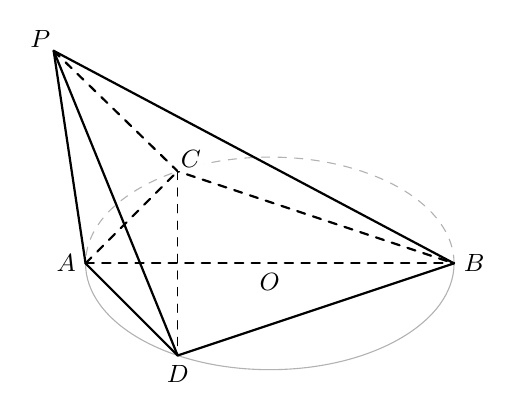
\begin{tikzpicture}[scale=0.9,line cap=round,line join=round]
  \coordinate (A) at (0,0);
  \coordinate (B) at (5.2,0);
  \coordinate (O) at (2.6,0);
  \coordinate (C) at (1.3,1.3);
  \coordinate (D) at (1.3,-1.3);
  \coordinate (P) at (-0.45,3.0);
  \draw[dashed,gray!60] (O) ++(2.6,0) arc[start angle=0, end angle=180, x radius=2.6, y radius=1.5];
  \draw[gray!60] (O) ++(-2.6,0) arc[start angle=180, end angle=360, x radius=2.6, y radius=1.5];
  \draw[thick,dashed] (A)--(B);
  \draw[thick] (A)--(P)--(B);
  \draw[thick,dashed] (P)--(C)--(B);
  \draw[thick] (P)--(D)--(B);
  \draw[thick,dashed] (A)--(C);
  \draw[thick] (A)--(D);
  \draw[dashed] (C)--(D);
  \node[left] at (A) {\small \(A\)};
  \node[right] at (B) {\small \(B\)};
  \node[below] at (O) {\small \(O\)};
  \node[above right,fill=white,inner sep=1pt] at (C) {\small \(C\)};
  \node[below] at (D) {\small \(D\)};
  \node[above left,fill=white,inner sep=1pt] at (P) {\small \(P\)};
\end{tikzpicture}

{\small 图 10：压轴题的空间结构。\(C,D\) 关于 \(AB\) 对称，公共棱为 \(PB\)。}
\end{center}

\textbf{（1）证明 \(BC\perp PC\)。} 因为 \(AB\) 为圆直径，\(C\) 在圆上，所以 \(\angle ACB=\frac{\pi}{2}\)，即 \(BC\perp AC\)。又 \(PA\perp\) 底面，且 \(BC\) 在底面内，所以 \(PA\perp BC\)。直线 \(PA,AC\) 在平面 \(PAC\) 内相交，故
\[
BC\perp\text{平面 }PAC.
\]
由于 \(PC\subset\text{平面 }PAC\)，所以
\[
\boxed{BC\perp PC}.
\]

\textbf{基本长度。} 圆半径 \(OA=OC=3\)，且 \(\angle AOC=\frac{\pi}{3}\)，所以 \(\triangle AOC\) 为等边三角形，\(AC=3\)。由直角三角形 \(ABC\)：
\[
BC=\sqrt{AB^2-AC^2}=\sqrt{36-9}=3\sqrt3.
\]
又
\[
PC=\sqrt{PA^2+AC^2}=5,\qquad
PB=\sqrt{PA^2+AB^2}=2\sqrt{13}.
\]
由对称性 \(PD=5,BD=3\sqrt3\)。

\textbf{（2）（i）二面角余弦。} 设 \(AB\) 与 \(CD\) 交于 \(E\)。过 \(C\) 作 \(CF\perp PB\)，垂足为 \(F\)。因为 \(C,D\) 关于平面 \(PAB\) 对称，\(PB\subset\text{平面 }PAB\)，所以对应地有
\[
DF\perp PB,\qquad DF=CF.
\]
因此 \(\angle CFD\) 是二面角 \(C-PB-D\) 的平面角。

在直角三角形 \(PBC\) 中，斜边上的高
\[
CF=\frac{PC\cdot BC}{PB}
=\frac{5\cdot3\sqrt3}{2\sqrt{13}}
=\frac{15\sqrt3}{2\sqrt{13}}.
\]
又 \(C,D\) 关于 \(AB\) 对称，故 \(E\) 是 \(CD\) 中点，且 \(CE\perp AB\)。在直角三角形 \(ABC\) 中，斜边上的高
\[
CE=\frac{AC\cdot BC}{AB}
=\frac{3\cdot3\sqrt3}{6}
=\frac{3\sqrt3}{2}.
\]
因 \(CE\perp AB\) 且 \(CE\perp PA\)，故 \(CE\perp\text{平面 }PAB\)，从而 \(CE\perp EF\)。在直角三角形 \(CEF\) 中
\[
\sin\angle CFE=\frac{CE}{CF}
=\frac{\frac{3\sqrt3}{2}}{\frac{15\sqrt3}{2\sqrt{13}}}
=\frac{\sqrt{13}}5.
\]
等腰三角形 \(CFD\) 中 \(FE\) 为顶角平分线，所以
\[
\angle CFD=2\angle CFE.
\]
由倍角公式
\[
\cos\angle CFD=1-2\sin^2\angle CFE
=1-2\left(\frac{\sqrt{13}}5\right)^2
=-\frac1{25}.
\]
故
\[
\boxed{\cos\angle(C-PB-D)=-\frac1{25}}.
\]

\begin{center}
\begin{tikzpicture}[scale=0.95]
  \coordinate (P) at (0,2.7);
  \coordinate (B) at (4.3,0);
  \coordinate (C) at (0,0);
  \coordinate (M) at ($(P)!0.666!(B)$);
  \coordinate (N) at ($(P)!0.8!(C)$);
  \coordinate (Q) at ($(M)!0.55!(N)$);
  \draw[thick] (P)--(B)--(C)--cycle;
  \draw[thick] (M)--(N);
  \draw[dashed] (P)--(Q);
  \fill (P) circle (1.4pt) node[above] {\small \(P\)};
  \fill (B) circle (1.4pt) node[right] {\small \(B\)};
  \fill (C) circle (1.4pt) node[left] {\small \(C\)};
  \fill (M) circle (1.4pt) node[below right] {\small \(M\)};
  \fill (N) circle (1.4pt) node[left] {\small \(N\)};
  \fill (Q) circle (1.4pt) node[below] {\small \(Q\)};
  
\end{tikzpicture}

{\small 图 11：体积条件把 \(Q\) 的轨迹压缩到 \(\triangle PBC\) 内的一条线段 \(MN\)。}
\end{center}

\textbf{（2）（ii）最小距离。} 由对称性
\[
S_{ACBD}=2S_{\triangle ABD},
\]
故
\[
V_{Q-ACBD}=2V_{Q-ABD}.
\]
题设 \(V_{Q-PAD}=V_{Q-ACBD}\)，所以
\[
V_{Q-PAD}=2V_{Q-ABD}.
\]
换顶点看体积：
\[
V_{Q-PAD}=V_{P-ADQ},\qquad V_{Q-ABD}=V_{B-ADQ}.
\]
两四面体同底 \(\triangle ADQ\)，体积比等于高之比。设平面 \(ADQ\) 与 \(PB\) 交于 \(M\)，则
\[
PM:MB=2:1,\qquad PM=\frac23PB=\frac{4\sqrt{13}}3.
\]

另一方面，
\[
S_{ACBD}=4S_{\triangle ACD},
\]
故同理设平面 \(ADQ\) 与 \(PC\) 交于 \(N\)，则
\[
PN:NC=4:1,\qquad PN=\frac45PC=4.
\]
由于 \(M,N\) 同时在平面 \(ADQ\) 与平面 \(PBC\) 内，二者交线为 \(MN\)。又 \(Q\in \triangle PBC\) 及其内部，故
\[
Q\in MN.
\]
问题转化为在线段 \(MN\) 上取点 \(Q\)，求 \(|PQ|\) 的最小值，即求点 \(P\) 到线段 \(MN\) 的距离。

在直角三角形 \(PBC\) 中
\[
\cos\angle BPC=\frac{PC}{PB}=\frac5{2\sqrt{13}}.
\]
由余弦定理
\[
MN^2=\left(\frac{4\sqrt{13}}3\right)^2+4^2
-2\cdot\frac{4\sqrt{13}}3\cdot4\cdot\frac5{2\sqrt{13}}
=\frac{112}{9},
\]
故
\[
MN=\frac{4\sqrt7}{3}.
\]
面积比为
\[
\frac{S_{\triangle PMN}}{S_{\triangle PBC}}
=\frac{PM}{PB}\cdot\frac{PN}{PC}
=\frac23\cdot\frac45=\frac8{15}.
\]
又
\[
S_{\triangle PBC}=\frac12\cdot PC\cdot BC
=\frac12\cdot5\cdot3\sqrt3
=\frac{15\sqrt3}{2},
\]
所以
\[
S_{\triangle PMN}=4\sqrt3.
\]
设点 \(P\) 到 \(MN\) 的距离为 \(h\)，则
\[
4\sqrt3=\frac12\cdot \frac{4\sqrt7}{3}\cdot h,
\]
得
\[
h=\frac{6\sqrt{21}}7.
\]
垂足落在线段 \(MN\) 内，因此最小值为
\[
\boxed{|PQ|_{\min}=\frac{6\sqrt{21}}7}.
\]


}
\switchcolumn
\teachblock{压轴题讲法}{
第 19 题不要一上来堆计算。建议按四层板书：第一层用圆周角和线面垂直证 \(BC\perp PC\)；第二层补齐长度；第三层用对称构造二面角平面角；第四层把体积相等转成 \(PM:MB=2:1\)、\(PN:NC=4:1\)，再降为平面最值。
}
\teachblock{课堂讲评建议}{
\begin{enumerate}[leftmargin=2em]
  \tightlist
  \item 基础题不要只报答案，要追问“为什么触发这个模型”。例如正方体外接球触发体对角线，圆台触发轴截面。
  \item 多选题要训练反例意识。第 10 题适合让学生自己画两个垂直平面，找出 D 的反例。
  \item 图像题要补图。第 16 题若没有图像重构，学生容易只背公式，不能解释相位符号。
  \item 立体几何要双路径。几何法适合课堂呈现，向量法适合校验和补救。
  \item 压轴题要分段讲。第 19 题最难处不是计算，而是把体积条件翻译为 \(Q\) 的轨迹。
\end{enumerate}
}
\end{paracol}

\section{全卷方法模型总表}

\begin{center}
\begin{tabularx}{\linewidth}{>{\bfseries}p{3.1cm}|X}
\toprule
模型 & 触发条件与操作\\
\midrule
定义域约束 & 出现 \(\tan x\)、根式、分式、对数时，先找无意义点或限制条件。\\
\midrule
三角图像读参 & 先读振幅 \(A\)，再由相邻零点或峰谷读周期，最后用穿越方向确定相位。\\
\midrule
向量基底法 & 选两条或三条独立方向作基底，把分点、投影、垂直、交点统一转成系数比较或点积。\\
\midrule
空间平移法 & 求异面直线角时，找中点或平行线，把异面角转到同一平面内。\\
\midrule
二面角平面角 & 围绕公共棱作两条垂线；若有对称结构，优先利用垂足对称与倍角关系。\\
\midrule
体积比转轨迹 & 同底体积比等于高比；高比沿一条相交直线转成分点比，最后得到点的轨迹线段。\\
\bottomrule
\end{tabularx}
\end{center}

\section{课堂讲评与终审评估}



\begin{warnbox}{终审结论}
本稿已修正原材料中两处易造成误读的符号：第 17 题写为 \(AB=\sqrt2\,AA_1\)，第 18 题写为 \(a\cos C+\sqrt3\,c\sin A=b+2c\)。数学结论与原答案一致。

版式上按 A4 教师讲评稿处理，基础题压缩呈现，函数图像与立体几何题补入示意图。若用于正式课堂，可优先讲第 6、7、9、16、17、19 题，其余题作为模型回扣与错因定位。
\end{warnbox}

\end{document}
